\documentclass{standalone}
\usepackage{tikz}
\usepackage{adjustbox}
\usepackage{helvet}  
\usepackage{sansmathfonts}  
\renewcommand{\familydefault}{\sfdefault}  
\usetikzlibrary{arrows.meta,calc,decorations.pathmorphing}
\usetikzlibrary{shapes.geometric, shapes.arrows}
\usepackage{xcolor}

\definecolor{color001122}{HTML}{001122}
\begin{document}
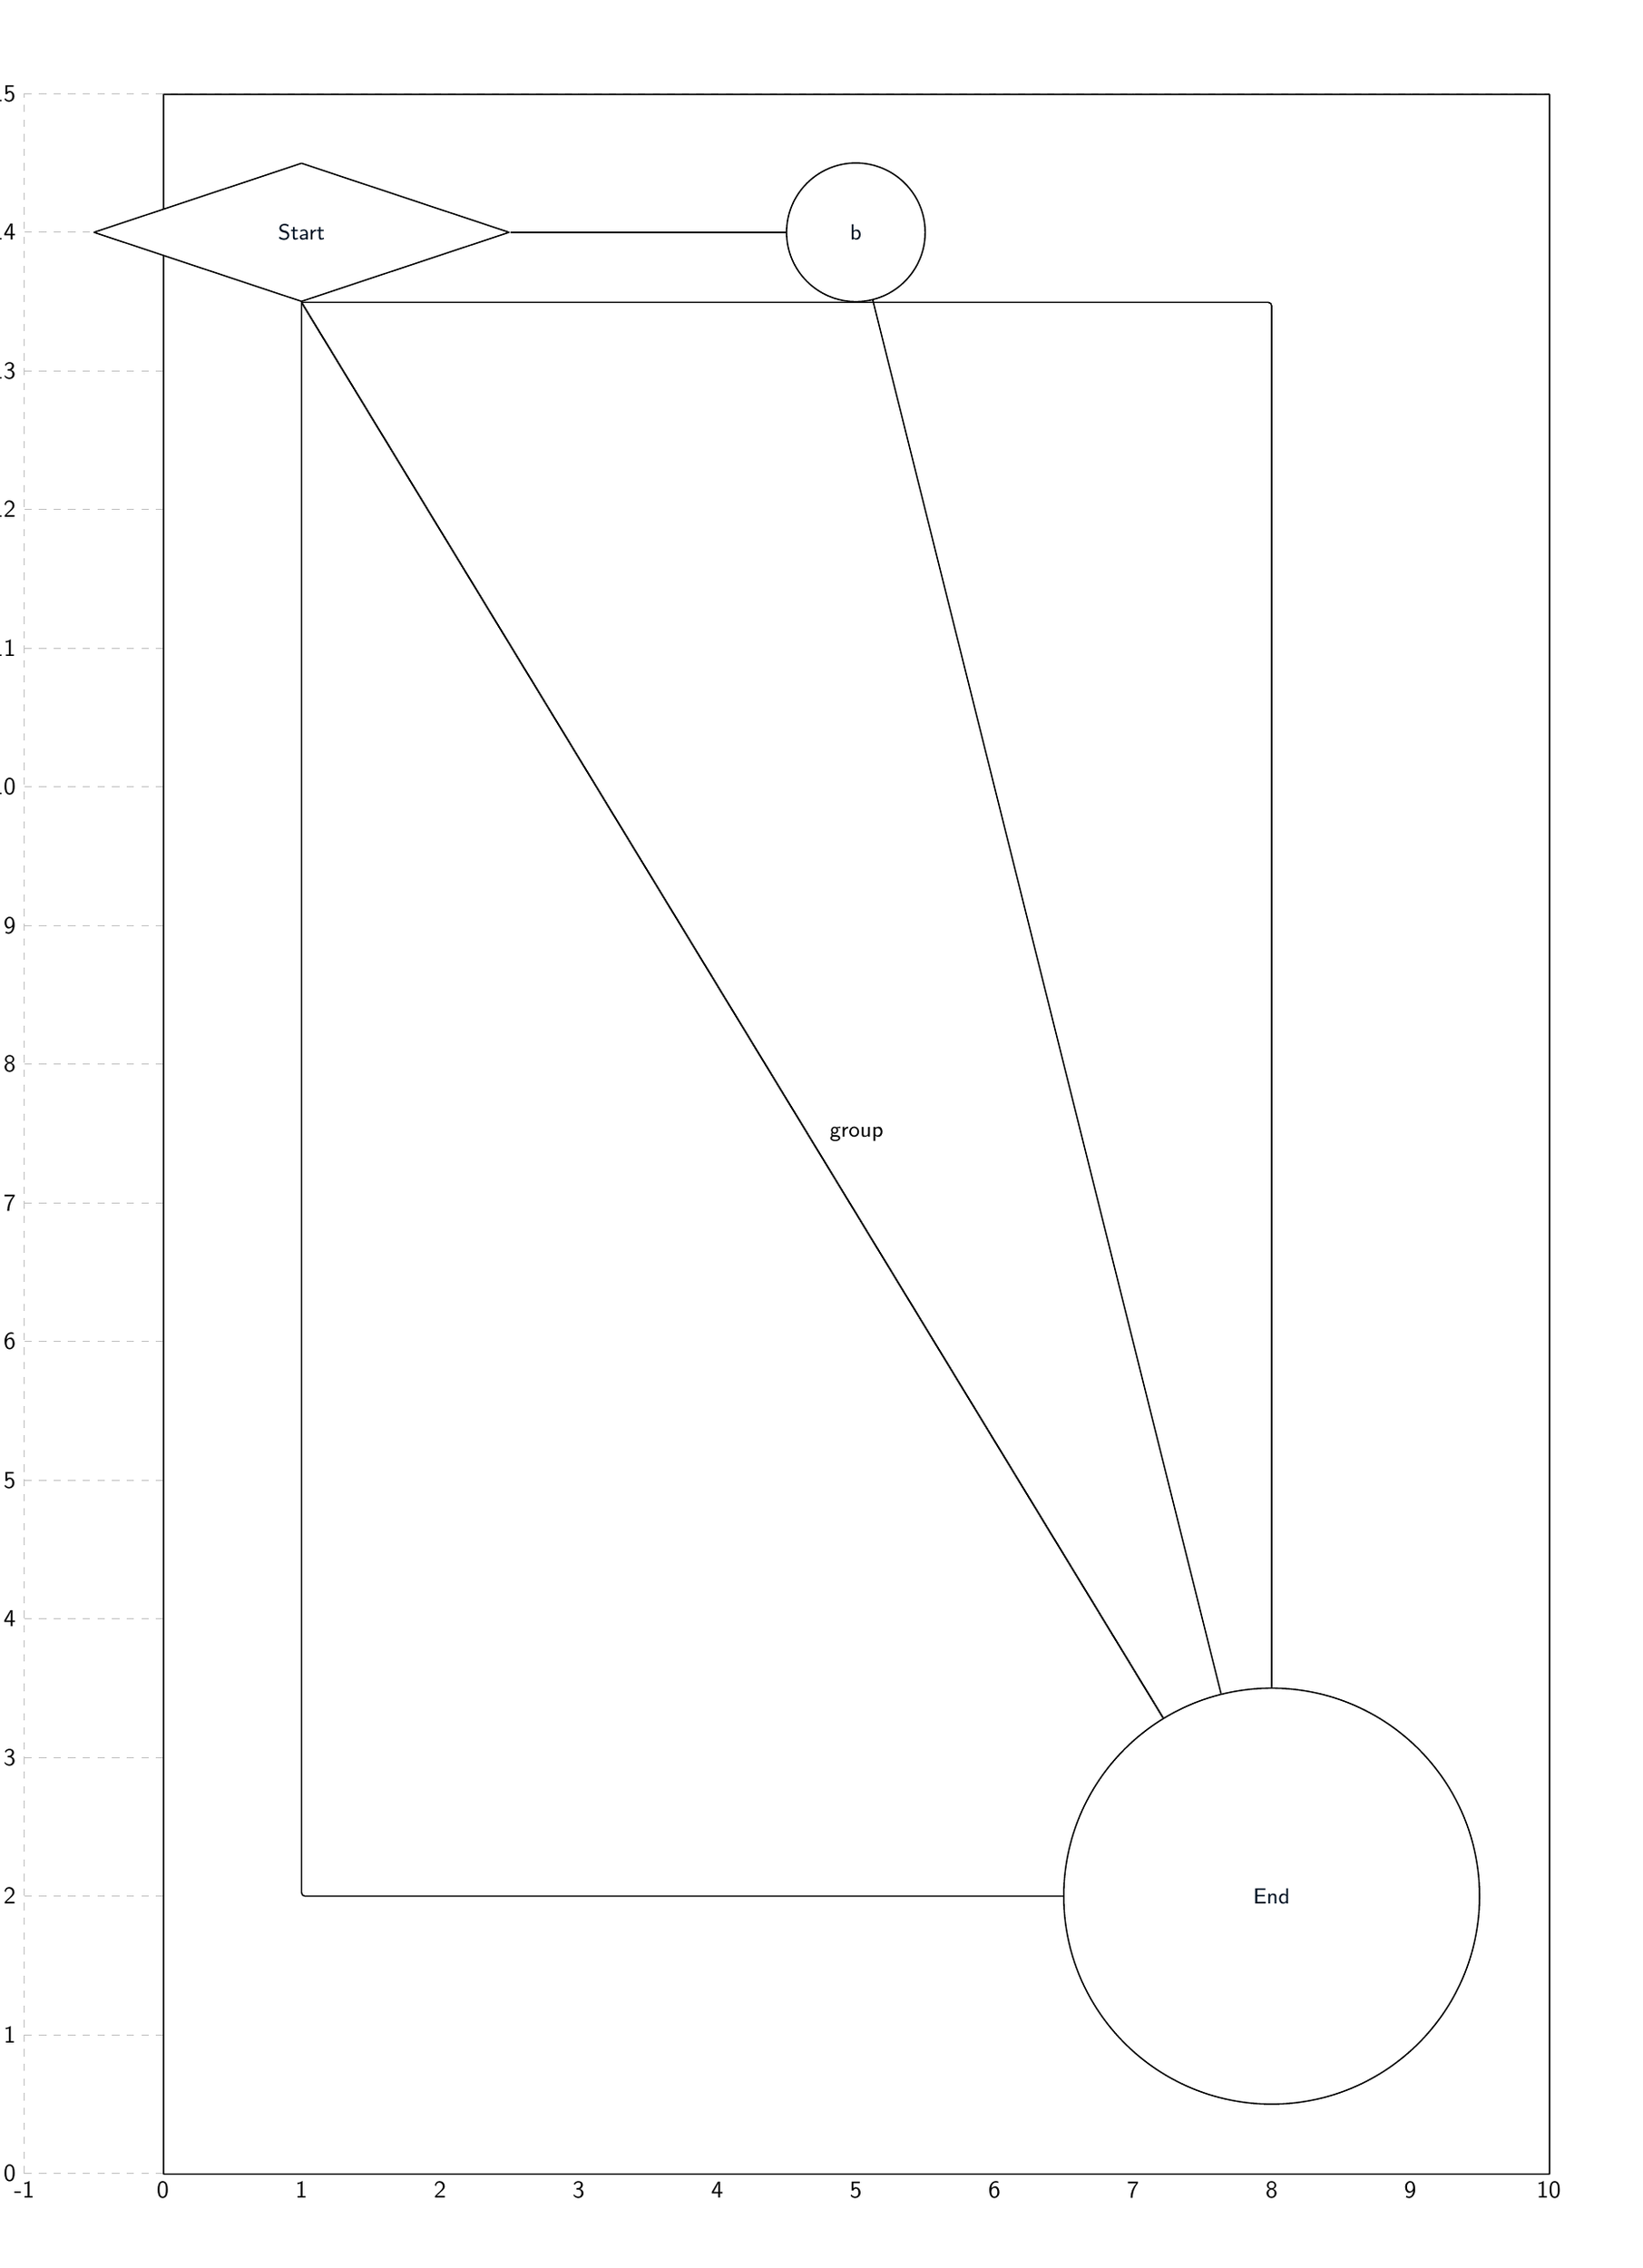
\begin{tikzpicture}
\useasboundingbox (-2,-1) rectangle (21,31);



\draw[dashed,gray,opacity=0.5] (-2,0) -- (-2,30);
\node[below] at (-2,0) {-1};
\draw[dashed,gray,opacity=0.5] (0,0) -- (0,30);
\node[below] at (0,0) {0};
\draw[dashed,gray,opacity=0.5] (2,0) -- (2,30);
\node[below] at (2,0) {1};
\draw[dashed,gray,opacity=0.5] (4,0) -- (4,30);
\node[below] at (4,0) {2};
\draw[dashed,gray,opacity=0.5] (6,0) -- (6,30);
\node[below] at (6,0) {3};
\draw[dashed,gray,opacity=0.5] (8,0) -- (8,30);
\node[below] at (8,0) {4};
\draw[dashed,gray,opacity=0.5] (10,0) -- (10,30);
\node[below] at (10,0) {5};
\draw[dashed,gray,opacity=0.5] (12,0) -- (12,30);
\node[below] at (12,0) {6};
\draw[dashed,gray,opacity=0.5] (14,0) -- (14,30);
\node[below] at (14,0) {7};
\draw[dashed,gray,opacity=0.5] (16,0) -- (16,30);
\node[below] at (16,0) {8};
\draw[dashed,gray,opacity=0.5] (18,0) -- (18,30);
\node[below] at (18,0) {9};
\draw[dashed,gray,opacity=0.5] (20,0) -- (20,30);
\node[below] at (20,0) {10};
\draw[dashed,gray,opacity=0.5] (-2,0) -- (20,0);
\node[left] at (-2,0) {0};
\draw[dashed,gray,opacity=0.5] (-2,2) -- (20,2);
\node[left] at (-2,2) {1};
\draw[dashed,gray,opacity=0.5] (-2,4) -- (20,4);
\node[left] at (-2,4) {2};
\draw[dashed,gray,opacity=0.5] (-2,6) -- (20,6);
\node[left] at (-2,6) {3};
\draw[dashed,gray,opacity=0.5] (-2,8) -- (20,8);
\node[left] at (-2,8) {4};
\draw[dashed,gray,opacity=0.5] (-2,10) -- (20,10);
\node[left] at (-2,10) {5};
\draw[dashed,gray,opacity=0.5] (-2,12) -- (20,12);
\node[left] at (-2,12) {6};
\draw[dashed,gray,opacity=0.5] (-2,14) -- (20,14);
\node[left] at (-2,14) {7};
\draw[dashed,gray,opacity=0.5] (-2,16) -- (20,16);
\node[left] at (-2,16) {8};
\draw[dashed,gray,opacity=0.5] (-2,18) -- (20,18);
\node[left] at (-2,18) {9};
\draw[dashed,gray,opacity=0.5] (-2,20) -- (20,20);
\node[left] at (-2,20) {10};
\draw[dashed,gray,opacity=0.5] (-2,22) -- (20,22);
\node[left] at (-2,22) {11};
\draw[dashed,gray,opacity=0.5] (-2,24) -- (20,24);
\node[left] at (-2,24) {12};
\draw[dashed,gray,opacity=0.5] (-2,26) -- (20,26);
\node[left] at (-2,26) {13};
\draw[dashed,gray,opacity=0.5] (-2,28) -- (20,28);
\node[left] at (-2,28) {14};
\draw[dashed,gray,opacity=0.5] (-2,30) -- (20,30);
\node[left] at (-2,30) {15};
\node[shape=rectangle, fill=white, draw=black, minimum width=20cm, minimum height=30cm, rounded corners=0.005cm, line width=0.02cm, text opacity=1, font=\footnotesize, inner sep=0pt, anchor=north west] (group) at (0,30) {\adjustbox{max width=20cm, max height=30cm}{\small{\sffamily{group}}}};
\node[shape=diamond, fill=white, draw=black, minimum width=6cm, minimum height=2cm, rounded corners=0.005cm, line width=0.02cm, text opacity=1, font=\footnotesize, inner sep=0pt] (start) at (2,28) {\adjustbox{max width=6cm, max height=2cm}{\textcolor{color001122}{\small{\sffamily{Start}}}}};
\node[shape=circle, fill=white, draw=black, minimum width=6cm, minimum height=6cm, rounded corners=0.005cm, line width=0.02cm, text opacity=1, font=\footnotesize, inner sep=0pt] (end) at (16,4) {\adjustbox{max width=6cm, max height=6cm}{\textcolor{color001122}{\small{\sffamily{End}}}}};
\node[shape=circle, fill=white, draw=black, minimum width=2cm, minimum height=2cm, rounded corners=0.005cm, line width=0.02cm, text opacity=1, font=\footnotesize, inner sep=0pt] (b) at (10,28) {\adjustbox{max width=2cm, max height=2cm}{\textcolor{color001122}{\small{\sffamily{b}}}}};
\draw[draw=black, line width=0.02cm, rounded corners=0.05cm] (start) -- (b);
\draw[draw=black, line width=0.02cm, rounded corners=0.05cm] (b) -- (end);
\draw[draw=black, line width=0.02cm, rounded corners=0.05cm] (start.south) -- (end);
\draw[draw=black, line width=0.02cm, rounded corners=0.05cm] (start.south) -- (end);
\draw[draw=black, line width=0.02cm, rounded corners=0.05cm] (start.south) |- (end);
\draw[draw=black, line width=0.02cm, rounded corners=0.05cm] (start.south) -| (end);

\end{tikzpicture}
\end{document}